\chapter{Software Construction}

Bei der Entwicklung von Software gibt es diverse Prozesse. Weit verbreitet sind das Wasserfall-, Scrum- und Kanban Modell. Obwohl diese nicht spezifisch für die Domäne der Webentwicklung sind, sollen sie kurz beschrieben werden.

Danach wird vorgestellt, wie \Gls{glos:htmlLabel} Dokumente korrekt erstellt werden und zum Schluss welche Programmiersprachen in der Webentwicklung eingesetzt werden.

\section{Vorgehensmodelle}
Für \gls{kmuLabel} Unternehmen haben sich in der Webentwicklung drei Vorhersagemodelle etabliert. Das Wasserfall, Scrum und Kanban Modell. 

\subsection{Wasserfallmodell}
Ersteres ist ein strikt lineares (nicht iteratives) Model in welchem eine Phase nach der anderen Abgearbeitet wird. Das Ergebnis der vorherigen Phase fliesst dabei in die nächste mit ein. Das vorgehen ist sehr starr, da alles was zu beginn definiert wurde während des Projektes nicht mehr angepasst werden kann.

\begin{figure}[H]
  \centering
  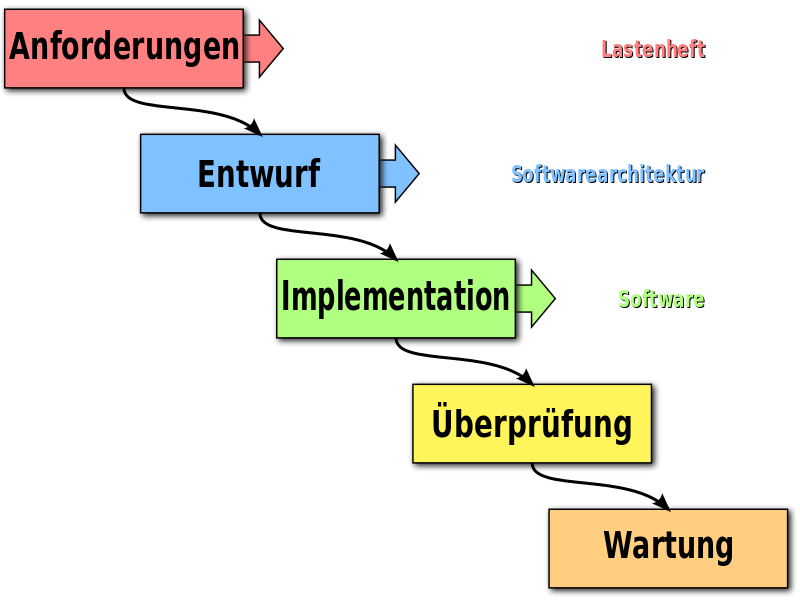
\includegraphics[width=0.6\textwidth]{images/wasserfall.png}
  \caption{Wasserfallmodel\footcite{Waterfall_model-de_-_Wasserfallmodell__Wikipedia_2015-06-03}}
  \label{fig:softwareconstruction:vorgehensmodelle:wasserfall}
\end{figure}

\subsection{Scrum}
Scrum hat sich zum Ziel gesetzt, den Kunden früher in den Entwicklungsprozess mit einzubeziehen. 
Durch eine iterative Vorgehensweise hat der Kunde regelmässig die Möglichkeit, Einfluss zu nehmen. 

\begin{figure}[H]
  \centering
  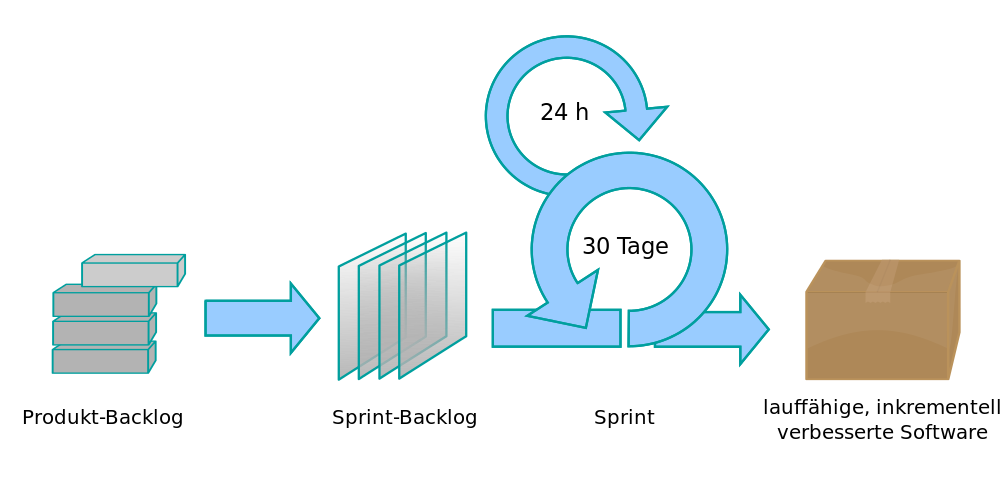
\includegraphics[width=0.8\textwidth]{images/scrum.png}
  \caption{Scrum\footcite{Scrum_process-de_-_Scrum__Wikipedia_2015-06-03}}
  \label{fig:softwareconstruction:vorgehensmodelle:scrum}
\end{figure}

Eine Iteration wird als Sprint bezeichnet. Er sollte nicht länger als 30 Tage dauern und an dessen Ende sollte stets eine lauffähige Version der Webseite vorgestellt werden können. Vor jedem Sprint hat der Kunde die Möglichkeit den Sprint-Backlog zu füllen. Dort sind die Arbeitspakete definiert, die in der nächsten Iteration umgesetzt werden sollen. Dadurch sieht der Kunde wie die Software sich entwickelt und kann entsprechend Einfluss nehmen.

\subsection{Kanban}
Kanban hat das primäre Ziel, ein Arbeitspaket so rasch fertigzustellen wie möglich. Dazu werden alle Arbeiten auf eine Karte geschrieben und an eine Tafel gehängt.

\begin{figure}[H]
  \centering
  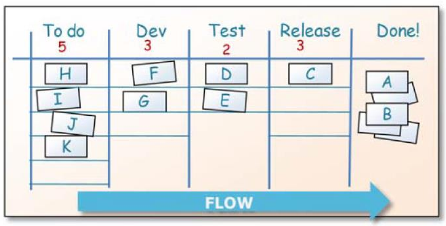
\includegraphics[width=0.8\textwidth]{images/kanban.png}
  \caption{Kanban}
  \label{fig:softwareconstruction:vorgehensmodelle:kanban}
\end{figure}

Jede Spalte hat eine Zahl welche definiert, wie viele Arbeitspakete auf einmal in einer Spalte liegen dürfen. Es wird gemessen, wie lange die Durchlaufzeit pro Paket ist und dann wird versucht, diese Zeit durch Prozessverbesserungen zu minimieren. 


\section{HTML}
Jede Webseite läuft mit \Gls{glos:htmlLabel}. Dabei handelt es sich um eine Auszeichnungssprache für digitale Dokumente. Sie definiert die Struktur und den Aufbau einer Webseite.

Der Aufbau wird von dem \gls{w3cLabel} definiert:
\begin{lstlisting}
<!DOCTYPE html>
<html>

<head>
<meta charset="UTF-8">
<title>Title of the document</title>
</head>

<body>
Content of the document......
</body>

</html> 
\end{lstlisting}

Aufgebaut ist das Dokument über Tags, welche zwischen den < und > Zeichen definiert sein. Der \textit{DOCTYPE} gibt die \Gls{glos:htmlLabel} Version an. Im \textit{head} werden Kopfdaten definiert. Zum Beispiel der Titel der Seite oder die Schlüsselwörter, welche von den Suchmaschinen gefunden werden sollen. Und schlussendlich wird im \textit{body} der Inhalt der Seite angegeben.

Im \textit{body} können weitere Tags definiert werden. Zum Beispiel können Tabellen erzeugt werden. Der folgende Code

\begin{center}
    \begin{tabular}{| l | l | l | l |}
    \hline
	Zelle 1 & Zelle 2 & Zelle 3 \\ \hline
	Zelle 4 & Zelle 5 & Zelle 6 \\ \hline
	Zelle 7 & Zelle 8 & Zelle 9 \\ \hline
    \end{tabular}
\end{center}

wird folgendermassen definiert:

\begin{lstlisting}
<table>
	<tr>
		<td>Zelle 1</td>
		<td>Zelle 2</td>
		<td>Zelle 3</td>
	</tr>
	<tr>
		<td>Zelle 4</td>
		<td>Zelle 5</td>
		<td>Zelle 6</td>
	</tr>
	<tr>
		<td>Zelle 7</td>
		<td>Zelle 8</td>
		<td>Zelle 9</td>
	</tr>
</table>
\end{lstlisting}

Eingeleitet wird die Tabelle mittels \textit{<table>} begonnen und mit \textit{</table>} wieder beendet. Eine Reihe wird mit \textit{<tr>} definiert und eine Zelle mit \textit{<td>}

Über die Tabellenstruktur kann der gesamte Aufbau einer Seite gesteuert werden. Für eine professionelle Entwicklung und eine gute Suchmaschinen Unterstützung ist dies jedoch nicht empfehlenswert, denn nicht jede Seite ist automatisch eine Tabelle. Möchte man einen Textabsatz definieren, sollte man zum Beispiel den <p> Tag (paragraph) verwenden. Dabei spricht man von semantischen \Gls{glos:htmlLabel}. Suchmaschinen wissen dann, dass es sich dabei um einen Textabsatz handelt und nicht um eine Tabelle.

Die der Schwierigkeitsgrad von \Gls{glos:htmlLabel} ist sehr niedrig. Jedoch ist das umsetzen von einer semantisch korrekten Seite um Faktoren schwerer zu bewerkstelligen.

\section{Programmiersprachen}
Da das Web auf einer  Client-/Server-Architektur aufbaut gibt es Programmiersprachen für beide Seiten. Eine Webseite besteht Grundsätzlich aus \Gls{glos:htmlLabel} Code, welcher von weiteren Clienten-Seitigen Programmiersprachen manipuliert werden kann. Die Server-Seitigen Sprachen haben hingegen das primäre Ziel, \Gls{glos:htmlLabel} oder Client-Seitigen Code zu generieren.

Es gibt unzählige Programmiersprachen. Folgend eine Liste der populärsten Server-Programmiersprachen gemäss dem TIOBE Index\footcite{TIOBE_Software_Tiobe_Index_2015-06-04}.

\begin{itemize}
\item Java
\item C
\item C++
\item C\#
\item Phyton
\end{itemize}

Die einzige verbreitete Programmiersprache für die Benutzung im Browser is JavaScript. Es gibt alternativen mit ActionScript, mit welchem Flash-Dateien umgesetzt werden, oder Java um Java Applets zu programmieren. Die beiden Varianten verlieren jedoch immer mehr an Bedeutung, wie dem TIOBE Index entnommen werden kann.

Es gibt Sprachen, welche in JavaScript transcodiert werden. Zum Beispiel \textit{Coffee Script} oder \textit{Dart}. Beim Transcodieren wandelt der Compiler die Sprache dann in valides JavaScript um.
t
Die Frage, welche Programmiersprache man einsetzen soll ist sehr schwierig zu beantworten da die Auswahl sehr gross ist. Folgende Punkte sollten dabei beachtet werden:
\begin{itemize}
\item Grösse und Komplexität der Software
\item Problemdomäne
\item Knowhow
\end{itemize}
Je nach Grösse und Komplexität spielt auch die Geschwindigkeit eine Rolle. Es gibt Sprachen die in diesem Bereich Vorteile besitzen wie C++ die sehr schnell sind.

Es ist möglich, alles in jeder Sprache umzusetzen. Nur eignen sich spezifische Sprachen für gewisse Arbeiten besser als andere. Zum Beispiel können mathematische Probleme mit funktionale Programmiersprachen wie Haskell oder F\#, einfacher und verständlicher gelöst werden. Deshalb sollte stets die passende Sprache ausgewählt werden.

Auch wenn die Problemdomäne wichtig ist, so sollte stets auch das Wissen der Programmierer berücksichtigt werden. Denn wer sich in einer Programmiersprache zuhause fühlt, der leistet auch bessere Arbeit.
